%!TEX root=paper.tex

  \section{Automated Outlier Detection and Monitoring}
  \label{sec:outliers}
  % \va{Shouldn't this be promoted to a section? It is neither utilization- nor performance- related. Either that, or Section~\ref{sec:user} should be folded into this section too, and then Sections~\ref{sec:version} and~\ref{sec:regression} merged into another section. Otherwise we have a very scattered paper}
  
  When an API endpoint is called from within a highly interactive application 
    (as it is the case with \epTranslationsColor in the previous section) 
  of particular interest to the API developers are {\em performance outliers}.   
  Indeed, a translation request that takes three times more than expected can   decrease the perceived quality of the application significantly. 
  Thus, identifying, collecting all appropriate data, and diagnosing the root   causes of such outliers is especially critical in improving application quality. 
    
  For this purpose the \tool tracks for every monitored endpoint a {\em running average} response time value.\footnote{
    For performance reasons, we assume that the response times for the endpoints are normally distributed. 
    Otherwise, more general density distribution information must be collected in real time.}
  When it detects that a given request is an outlier with respect to this past average running value\footnote{A configurable threshold with a default value of $2.5$ times the running average response time is used for this purpose}, it triggers the {\em outlier data collection routine} which stores extra information about the current execution environment. This extra data includes: the current Python stack trace, CPU load, memory consumption, request parameters, etc. 

  \begin{figure}[h!]
    \centering
    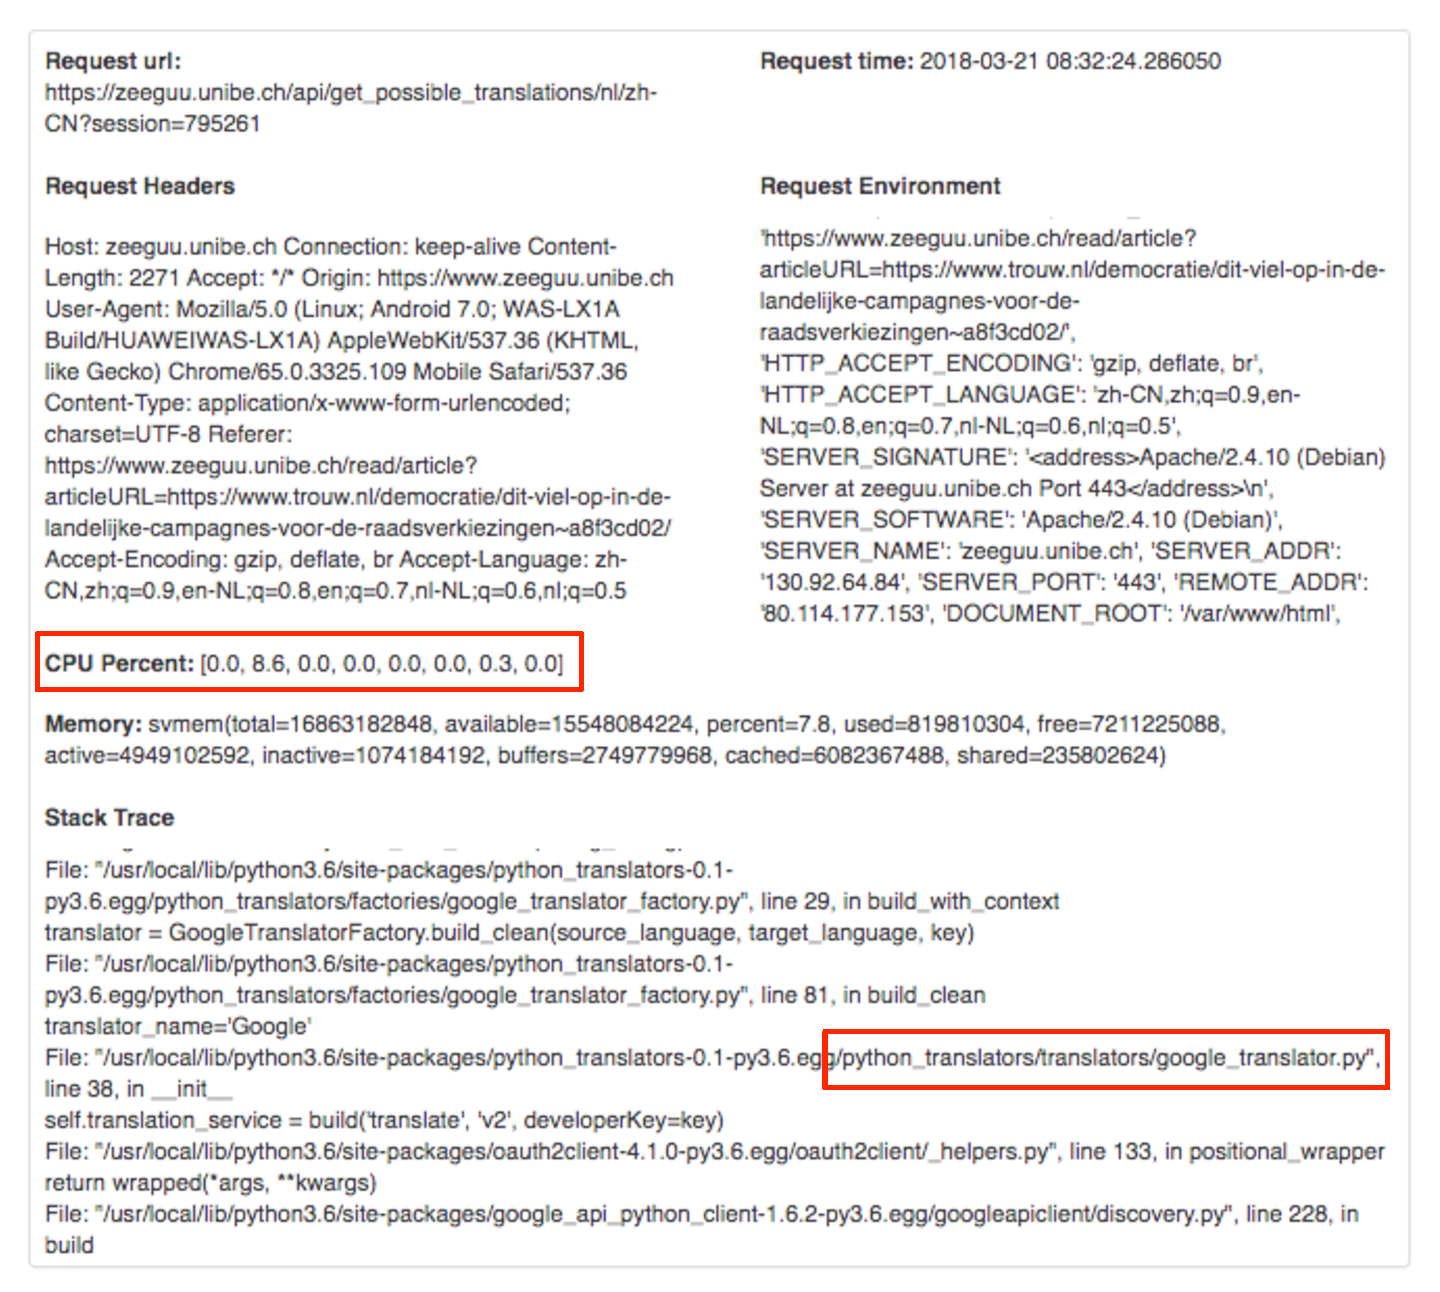
\includegraphics[width=\linewidth]{outlier-annotated}
    \caption{Automatically collected outlier information for the \epTranslationsColor endpoint}
    \label{fig:stack}
  \end{figure}
  
\Fref{fig:stack} shows an example of a \perspective{Performance Outlier Detail}  perspective on one of the outliers in the \epTranslationsColor endpoints. In this particular case, the analyst could corroborate several bits of informations: 

\begin{itemize}

  \item Neither the memory (1) nor the processor (2) were overloaded at the moment of the request. Thus the slow response is not due to the machine being overloaded.

  \item The stack trace snapshot shows that code was in the \code{google\_translator.py}. Since the system uses as back-end multiple translators it is revealing to see that in this particular case it was waiting for the Google Translator. By manually investigating multiple outliers, the developer discovered that in a large percentage of the cases the Google Translator was indeed the reason for the slow response time.

\end{itemize}

  \niceseparator

  In this way it is possible to get detailed insight into the operation of the application in the extreme cases without unnecessarily burdening it with logging this information for every request. 
  % In the discussion section we will come back and discuss some of the limitations of this approach.\ml{memento!}




